\subsection*{PARTIE I: développement binaire}
Question préliminaire.\newline
L'écriture proposée \emph{n'est pas un développement binaire} au sens de l'énoncé car $r_n=\frac{1}{2^n}$ alors que $r_n$ devrait être strictement plus petit que $\frac{1}{2^n}$. En effet :
\begin{displaymath}
 \frac{1}{2} + \frac{1}{2^2} + \cdots  + \frac{1}{2^n} =\frac{1}{2}\frac{1-\frac{1}{2^{n}}}{1-\frac{1}{2}}
= 1 - \frac{1}{2^{n}}
\end{displaymath}
Si $a$ admet un développement binaire à l'ordre $n$, comme chaque $d_i$ est inférieur ou égal à $1$ et $r_n<\frac{1}{2^n}$, on peut écrire
\begin{displaymath}
 a \leq 1+\frac{1}{2}+ \frac{1}{2^2}+\cdots+\frac{1}{2^n}+r_n
\leq \frac{1 - \frac{1}{2^{n+1}}}{1-\frac{1}{2}}   +r_n
= 2 - \frac{1}{2^n} +r_n <2
\end{displaymath}
\begin{enumerate}
 \item 
\begin{itemize}
 \item Si $a\in [0,1[$, $a=0+a$, donc $d_0=0$, $r_0=a$. 
 \item Si $a\in [1,2[$, $a=1 + (a-1)$, avec $a-1\in [0,1[$ donc $d_0=1$, $r_0=a-1$.
\end{itemize}

 \item On modifie le diagramme de l'énoncé en introduisant un compteur \verb|i|. On remplace la condition \verb|r>0| par une condition sur le compteur. On divise la variable \verb|r| par $2^n$ pour obtenir $r_n$ à la fin de l'exécution :
\begin{figure}[htp]
 \centering
 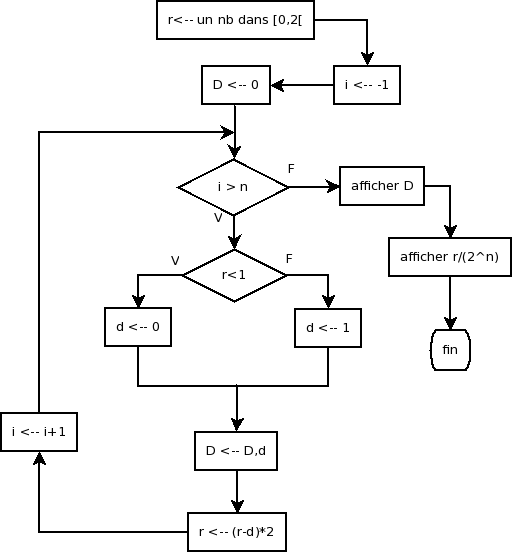
\includegraphics[width=8cm]{./Cbincos_1.png}
 % Cbincos_1.png: 513x553 pixel, 72dpi, 18.10x19.51 cm, bb=0 0 513 553
 \caption{reste et développement binaire à l'ordre $n$}
 \label{fig:Cbincos_1}
\end{figure}
\end{enumerate}


\subsection*{PARTIE II : itération d'une fonction}
\begin{enumerate}
 \item En étudiant une équation du second degré, on trouve rapidement que les points fixes de $f$ sont $1$ et $-\dfrac{1}{2}$.
 \item La fonction est décroissante dans $]-\infty,0]$ et croissante dans $[0,+\infty[$. Son graphe est une parabole.
\begin{figure}[ht]
 \centering
\input{Cbincos_2.pdf_t}
\label{fig:Cbincos_2}
\caption{graphe de $2x^2-1$}
\end{figure}
 
 \item
\begin{enumerate}
 \item L'étude de la fonction montre clairement que $[-1,1]$ est stable par $f$ c'est à dire que $x\in[-1,1]$ entraine $f(x)\in[-1,1]$. On en déduit que si $v_0$ est dans cet intervalle, tous les itérés $v_n$ y restent.
 \item Démonstration par récurrence. Pour $n=0$, on a bien $v_0 = \cos \theta$. Le passage de $n$ à $n+1$ vient de la formule pour $\cos(2x)$.
\begin{displaymath}
 v_n = \cos(2^n\theta)\Rightarrow 
v_{n+1}= 2 \cos^2(2^n\theta)-1 = \cos(2^{n+1}\theta)
\end{displaymath}
\end{enumerate}

\end{enumerate}

\subsection*{PARTIE III : suite de signes et développement binaire}
\begin{enumerate}
 \item
\begin{enumerate}
 \item Multiplions par $2^{n}$ le développement de $a$ à l'ordre n+1 :
\begin{displaymath}
 2^{n}a = \underset{\text{un nombre pair }= 2m}{\underbrace{2^{n}\left(d_0 + \frac{d_1}{2}+\cdots+\frac{d_{n-1}}{2^{n-1}} \right)}}
+ d_n + \frac{1}{2}d_{n+1}+
\underset{= h}{\underbrace{2^{n}r_{n+1}}} 
\end{displaymath}
avec $0\leq h < \frac{1}{2}$. On obtient bien la forme annoncée.
 \item D'après la valeur de $v_0$ et l'expression de $v_n$ avec des $\cos$, on obtient :
\begin{multline*}
 v_{n+1} = \cos(2^{n+1}\frac{a\pi}{2})= \cos(2^na\pi)
=\cos(2m\pi +d_n\pi + d_{n+1}\frac{\pi}{2} + h\pi)\\
= (-1)^{d_n}\cos(d_{n+1}\frac{\pi}{2} + h\pi)
\end{multline*}
On peut alors former un tableau des expressions de $v_{n+1}$
\begin{center}
\renewcommand{\arraystretch}{1.5}
\begin{tabular}{|c|c|c|} \hline
$d_n \backslash d_{n+1}$ & 0             & 1             \\ \hline
0                        & $\cos(h\pi)$  & $-\sin(h\pi)$ \\ \hline
1                        & $-\cos(h\pi)$ & $\sin(h\pi)$  \\ \hline
\end{tabular}
\end{center}

 \item Dans cette question, $h$ est compris strictement entre $0$ et $\frac{1}{2}$ donc les $\sin$ et $\cos$ intervenant dans le tableau précédent sont strictement positifs ce qui entraine
\begin{displaymath}
 (-1)^{d_n+d_{n+1}}v_{n+1}>0
\end{displaymath}

\end{enumerate}

 \item \`A partir de $a$, on peut trouver $d_0$. On forme alors $v_0$ puis la suite des $v_n$. On définit une suite $s_n$ en posant:
\begin{displaymath}
 s_n = \left\lbrace 
\begin{aligned}
 1&\text{ si } v_n<0 \\
 0&\text{ si } v_n>0 
\end{aligned}
\right. 
\end{displaymath}
On exclut ici le cas où $v_n=0$ \footnote{qui correspond à un nombre binaire ,le processus s'arrete alors au pas suivant}. La question c. se traduit par 
\begin{displaymath}
 s_{n+1}= d_n + d_{n+1}
\end{displaymath}
 On peut donc déduire $d_1$ de $s_1$ et $d_0$ puis $d_2$ de $s_2$ et $d-1$ et ainsi de suite. On remarque en particulier que si $v_{n+1}>0$, $d_n=d_{n+1}$ et qu'ils sont de valeur distinctes dans le cas négatif. On présente cet algorithme dans le schéma suivant :
\begin{figure}[htp]
 \centering
 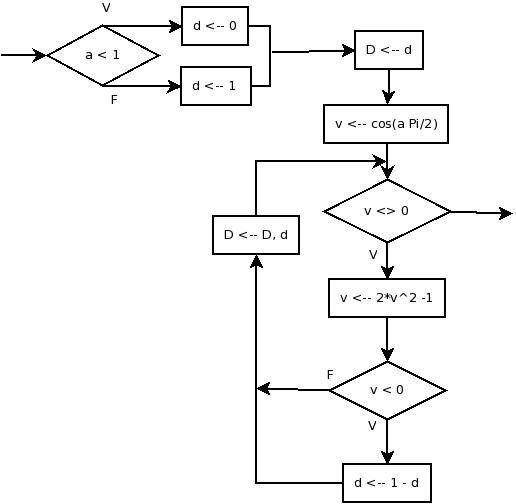
\includegraphics[width=8cm]{./Cbincos_3.png}
 % Cbincos_1.png: 513x553 pixel, 72dpi, 18.10x19.51 cm, bb=0 0 513 553
 \caption{signes et développement binaire}
 \label{fig:Cbincos_3}
\end{figure}

\item Si $a =\frac{2}{3}<1$, alors $d_0=0$
\begin{align*}
 &v_{0} = \cos \frac{\pi }{3} = \frac{1}{2} >0 \\
 &v_{1}= -\frac{1}{2}<0 \Rightarrow 1 = d_0 + d_1 \Rightarrow d_1 = 1 \\ 
 &v_{2}= -\frac{1}{2}<0 \Rightarrow 1 = d_1 + d_2 \Rightarrow d_1 = 0 \\
\end{align*}
et la suite ne change plus de valeur (point fixe de $f$). On en d{\'e}duit $d_{0}=0$, $d_{1}=1$, $d_{2}=0$,
$d_{3}=1$ et ainsi de suite alternativement.

\item Supposons $a=\frac{p}{q}$ et notons $\omega = e^{\frac{ia\pi}{2}}$. Ce nombre complexe est une racine $4q$-ieme de l'unité. Notons $N=4q$. Le complexe $\omega$ est dans le groupe $\U_N$, toutes ses puissances restent dans ce groupe. En particulier celles dont l'exposant est une puissance de $2$. Comme cet ensemble est \emph{fini}, il est impossible que toutes ces puissances soient deux à deux distinctes. Il existe donc deux entiers $i<j$ tels que
\begin{displaymath}
 w^{2^i} = w^{2^j} \Rightarrow w^{2^{i+1}}= \left( w^{2^i} \right)^2 = \left( w^{2^j}\right)^2  = w^{2^{j+1}} \Rightarrow \cdots
\end{displaymath}
Posons alors $m = i$ et $u=j-i$, on a
\begin{displaymath}
 \forall n\in \N : n\geq m \Rightarrow w^{2^{n+u}} = w^{2^n} 
\end{displaymath}
 Or la suite des $v_n$ est formée par les parties réelles de cette suite de puissance. Elle vérifie donc la même relation ainsi que la suite des $d_n$ qui s'en déduit par la méthode de la question 2.
\end{enumerate}
